\chapter{The continuum Schwinger model}\label{ch:SchingerContinuum}


%---------SECTION--------%


\section{Motivation and Introduction}\label{sec:Motivation1}


Quantum electrodynamics in $1+1$ dimensions with massless fermions was a model first studied by Schwinger in 1962 \cite{Schwinger1962} and thus it was coined the Schwinger model. This model is completely solvable using operator methods as demonstrated by Lowenstein and Swieca \cite{Lowenstein1971} and shows very interesting physical phenomena such as anomalies, a massive vector boson generated via a dynamical Higgs mechanism and the presence of confinement analogous to quark confinement in QCD$_4$ \cite{Bertlman}.\\

Hence, this model is a rich playground as a toy model for studying more complex gauge theories such as QCD$_4$ or supersymmetric gauge theories. Additionally, due to its simplicity, the Schwinger model is the perfect theory to first approach the subtleties in field theory such as anomalies, $\theta$-vacua, bosonization, symmetry breaking and non-perturbative methods in quantum field theory \cite{abdalla, Bertlman}.\\

In this chapter, we introduce the continuum Schwinger model and study its Lagrangian and its Hamiltonian. We derive the equations of motion that give rise to the dynamics of the system. Special emphasis is made on the fact that the model simplifies greatly over its cousin QED$_4$ due to the simplicity of electrodynamics in $D=2$. We derive using only the equations of motion that this model has a massive electromagnetic Boson, with its mass being proportional to the electromagnetic coupling constant $q_e$. We also discuss the energetics of pair production in one spatial dimension, and how this gives rise to a background electric field which induces a critical behavior in the system. Such behavior is a consequence of a discontinuity in the vacuum energy density due to the background field.\\

Secondly, we explore the chiral anomaly of the model and derive its exact value using the path integral formalism. The anomaly appears as a consequence of the classical action having two symmetries, a gauge $U(1)$ symmetry and an axial $U_A(1)$ symmetry, which upon quantization come into conflict yielding an anomalous divergence of the Noether current associated to the $U_A(1)$. Furthermore, we comment how this anomaly is directly related to the topology of the theory and can be understood by invoking the Atiyah-Singer index theorem relating the index of the Dirac operator and the topological information of the $U(1)$ gauge group.\\

Finally, we explore how the anomaly presents itself as a non-trivial restructuring of the fermion energy levels and the effect this restructuring has on the physical spectrum of the theory and the conserved charges associated to the symmetries of the model. Moreover, we study how the anomaly can be understood as both an infrared and an ultraviolet phenomenon, which originates from the fermion levels crossing the vacuum energy level and the ultraviolet cutoff correspondingly.


%---------SECTION--------%


\section{Lagrangian, Hamiltonian and equations of motion}\label{sec:LagrangianHamiltonian}

As a first step let us study the Lagrangian of QED$_4$, the close cousin of the Schwinger model. The Lagrangian reads

\begin{equation}
\mathscr{L} =  \bar\psi (i\slashed{\partial} - m )\psi - \frac{1}{4} F_{\mu\nu}^2 - q_e \bar\psi\slashed{A}\psi.
\end{equation}

In $3+1$ dimensions the coupling constant is dimensionless having th value $q_e^2 = 4\pi/137$. In units in which $\hbar = c = 1$ we have

\begin{equation}
[M] = [L]^{-1}=[T]^{-1}.
\end{equation}

Thus we have that the action $S = \int\dd[2]{x} \mathscr{L}$ is dimensionless which implies $$[\mathscr L] = [M]^2.$$ The free Dirac Lagrangian $\mathscr{L}_{\text{Dirac}} = \bar\psi (i\slashed{\partial} - m )\psi$ implies that $$[\bar\psi\psi] = [M].$$ Also, the free Maxwell Lagrangian must satisfy $$[F_{\mu\nu}^2] = [(\dmu A_\nu - \dnu A_\mu)^2] = [M]^2,$$
which implies $$[A_\mu] = [M]^0.$$ Hence, the interaction Lagrangian must have dimensions $$\mathscr{L}_{\text{int}}=-q_e \bar\psi\slashed{A}\psi = [M]^2.$$

The previous dimensional analysis yields $$[M]^2 = [q_e][M] \Rightarrow [q_e]=[M].$$ In a later section, we will prove that the axial anomaly creates a mass-generating mechanism for the gauge vector Boson (the ``photon'') which in this model has a mass $m_\gamma^2 =q_e^2/\pi$. Thus in this theory, the Boson carrying the electromagnetic interaction has a mass which is proportional to the interaction coupling constant.\\

After this short detour, we can focus our attention on the Lagrangian for the Schwinger model

\begin{equation}
    \mathscr{L} =  \bar\psi (i\slashed{D})\psi - \frac{1}{4} F_{\mu\nu}^2,
    \label{eq:lagrangian}
\end{equation}

with the covariant derivative $D_\mu = \partial_\mu + iq_e A_\mu$. In 1+1 dimensional Minkowski space the metric $g_{\mu\nu}\,(\mu,\nu=0,1)$ is
\begin{equation}
   g = \mqty(\dmat[0]{1,-1}).
\end{equation}

The Dirac matrices fulfill 
\begin{equation}
    \acomm{\gmu}{\gnu} = 2 g^{\mu\nu}
\end{equation}

which implies that $$(\gamma^0)^2 = 1$$ $$(\gamma^1)^2 = -1$$ and $$\acomm{\gamma^0}{\gamma^1}=0.$$

Therefore we can choose one of the following representations for the gamma matrices

\begin{equation}
    \gamma^0 = \sigma^1 ,\quad\quad \gamma^1 = -i\sigma^2,\quad\quad \gamma_5 = \gamma^0 \gamma^1 =\sigma^3 ,\label{eq:gammarep1}
\end{equation}
 or 
\begin{equation}
    \gamma^0 = \sigma^3,\quad\quad \gamma^1 = -i\sigma^2,\quad\quad \gamma_5 = \gamma^0 \gamma^1 =\sigma^1 \label{eq:gammarep2}.
\end{equation}

Both this representations  imply that $$(\gamma_5)^2 = 1$$ and $$\acomm{\gamma_5}{\gmu}=0.$$

Let us now turn our attention towards the Lagrangian of the theory \eqref{eq:lagrangian} 

\begin{equation*}
    \mathscr{L} = \bar\psi (i\slashed{\partial})\psi - \frac{1}{4} \qty(\partial_\mu A_\nu - \partial_\nu A_\mu)^2 -q_e \bar\psi\gnu\psi A_\nu
\end{equation*}

To obtain the equations of motion for the theory we employ the Euler-Lagrange equations

\begin{equation}
    \partial_\mu \frac{\partial \mathscr{L}}{\partial(\partial_\mu \psi)} = \frac{\partial\mathscr{L}}{\partial \psi}.
\end{equation}

which yield the Dirac equation 

\begin{equation}
    \qty(i \slashed{D} - m )\psi = 0,
\end{equation}

 and
 
\begin{equation}
    \partial_\mu \frac{\partial \mathscr{L}}{\partial(\partial_\mu A_\nu)} = \frac{\partial\mathscr{L}}{\partial A_\nu},
\end{equation}

yielding Maxwell's equations $$\partial_\mu F^{\nu\mu} =-q_e \bar\psi\gnu\psi \overset{.}{=}-q_e J^\nu.$$ Hence, as in standard QED$_4$ we get

\begin{equation}
    \partial_\mu F^{\mu\nu} = q_e J^\nu.
    \label{eq:maxwellmotion}
\end{equation}

We can take the divergence of \eqref{eq:maxwellmotion} and using the fact that $F^{\mu\nu}$ is anti-symmetric we obtain the usual current conservation law

\begin{equation}
\partial_\nu\partial_\mu F^{\mu\nu} = 0 =q_e\, \partial_\nu J^\nu. 
\label{eq:currentcons}
\end{equation}

Let us also introduce the anti-symmetric tensor $\varepsilon_{\mu\nu}$ defined by $\varepsilon_{01} = -\varepsilon_{10} = 1$. The following relation is easily proved

\begin{equation*}
	\varepsilon^{\mu\nu} = g^{\mu \rho}\varepsilon_{\rho\sigma}g^{\sigma \nu} = \mqty(\admat[0]{-1,1})=-\varepsilon_{\mu\nu}.
\end{equation*}

Using this result we can prove the following very important relationship for the gamma matrices in two dimensions:

\begin{equation}
\gmu\gf = \varepsilon^{\mu\nu}\gamma_\nu
\label{eq:gammarel}
\end{equation}

\begin{equation*}
	\gmu\gf = \gmu\gamma^0\gamma^1 = 
	\begin{cases}
		(\gamma^0)^2\gamma^1 = \gamma^1 = -\gamma_1 = \varepsilon^{01}\gamma_1 = \varepsilon^{0\nu}\gamma_\nu\quad \text{for }\mu=0\\
		\gamma^1\gamma^0\gamma^1=-\gamma^0(\gamma^1)^2 = \gamma^0 = \gamma_0 = \varepsilon^{10}\gamma_0 = \varepsilon^{1\nu}\gamma_\nu\quad \text{for }\mu=1.
	\end{cases}
\end{equation*}

The relation \eqref{eq:gammarel} allows expressing the axial current as the dual of the current vector

\begin{equation}
J_5^\mu \overset{.}{=} \bar\psi\gmu\gf\psi = \varepsilon^{\mu\nu} \bar\psi\gmu\psi = \varepsilon^{\mu\nu}J_\nu \overset{.}{=}{}^\ast J^\mu.
\end{equation}

Now, to write the equations of motion for the dual field strength tensor and the dual current we can use the following identity:

\begin{equation}
F_{\mu\nu}  = \varepsilon_{\mu\nu} F_{01},
\end{equation}

since $F_{00}=F_{11}=0$ and $F_{01} = \varepsilon_{01}F_{01} = \varepsilon_{10}F_{10}$. Thus, the dual to the $F$-tensor is the following scalar

\begin{equation}
{}^\ast F = \frac{1}{2}\varepsilon^{\mu\nu} F_{\mu\nu} = \frac{1}{2}\varepsilon^{\mu\nu}\varepsilon_{\mu\nu}F_{01} = -F_{01},
\end{equation}

here we have used the fact that $\varepsilon^{\mu\nu}\varepsilon_{\mu\nu}=-\delta^\mu_\mu =-2$. This immediately tells us that

\begin{equation}
F_{\mu\nu} = - \varepsilon_{\mu\nu}{}^\ast F,
\end{equation}

consequently, this leads to a dual equation of motion for ${}^\ast F$, viz

\begin{equation}
\partial_\mu {}^\ast F = - q_eJ_\mu^5.
\label{eq:dualeom}
\end{equation}

In the following section, we will show that by using the anomalous divergence of the axial current due to the chiral anomaly we get the following equation

\begin{equation}
    \qty(\Box + \frac{q_e^2}{\pi}){}^\ast F=0.
    \label{eq:KGmass}
\end{equation}

Hence, as suggested at the beginning of the chapter, even at the level of the equations of motion we can see the appearance of a massive gauge Boson, the photon, whose mass is  $m_\gamma = e/\sqrt{\pi}.$\\

Let us now study the Hamiltonian of the Schwinger model. We can compute the Hamiltonian by first obtaining the canonical energy-momentum tensor as the conserved Noether current of spacetime translations, viz 

\begin{equation}
T^{\mu}_{\;\;\nu} =  \frac{\partial \mathscr{L}}{\partial(\partial_\mu \psi)}\partial_\nu \psi + \text{c.c} - \delta^{\mu}_{\;\;\nu}\mathscr{L}\label{eq:emtensor}.
\end{equation}

Since the Lagrangian \eqref{eq:lagrangian} only depends on $\partial_\mu \psi$ equation \eqref{eq:emtensor} yields the following energy-momentum tensor 

\begin{equation}
T^{\mu\nu} = i\bar\psi\gmu\partial^\nu\psi - g^{\mu\nu} \mathscr{L}.
\end{equation}

We can use the equations of motion to set $\mathscr{L}=0$, obtaining

\begin{equation}
T^{\mu\nu} = i\bar\psi\gmu\partial^\nu\psi.
\end{equation}

We can find the total energy of the field as

\begin{equation}
H = \int \dd[2]{x}T^{00} = \int \dd[2]{x}i\bar\psi\gamma^{0}\partial^{0}\psi = \int \dd[2]{x}\bar\psi(-i\gamma^{1}\partial^{1} + m)\psi,
\end{equation}

to obtain the last equality we have made use of the equations of motion and we have added a mass term for the sake of completeness.\\

The previous derivation of the Hamiltonian and the total energy of the field is all concerning the Dirac field. However, we are interested in the full energy-momentum tensor for the Schwinger model. This tensor is simply obtained by adding the energy density of the Electric field in (1+1)-dimensional space and replacing derivatives $\partial$ with covariant derivatives $D$. Furthermore, we can fix a gauge in which $A_0=0$, the field tensor becomes $F_{01} = -\partial_0A_1 = E$ and with this the Hamiltonian is written as

\begin{equation}
H = \int \dd[2]{x}\qty(-i\bar\psi\gamma^1(\partial_1 + iq_eA_1)\psi + m\bar\psi\psi + \frac{1}{2}E^2).\label{eq:SchHAmil}
\end{equation}

\subsection{The Schwinger model in a Background electric field}\label{ssec:BackgroundField}
If we fix a gauge such that $A_0 = 0$ Maxwell's equations \eqref{eq:maxwellmotion} reduce to single equation

\begin{equation}
\partial_x E = q_e J^0\label{eq:gauss}
\end{equation}

which is Gauss's law. Since we are working in 1 spatial dimension it is easy to integrate \eqref{eq:gauss}

\begin{equation}
E = q_e\int\dd{x}J^0(x) + \mathcal E,
\end{equation}

where $\mathcal{E}$ is a constant background field which we can imagine as being generated by a parallel plate capacitor at both ends of the one-dimensional universe. This background field induces a very interesting physical behavior that was first described by Sydney Coleman in a beautiful paper \cite{Coleman1976}. Coleman explains that we can analyze the effect of this background field by considering a particle-antiparticle pair separated by a distance $x$ as seen in figure \ref{fig:conf}. 


\begin{figure}[htb]
	\centering
	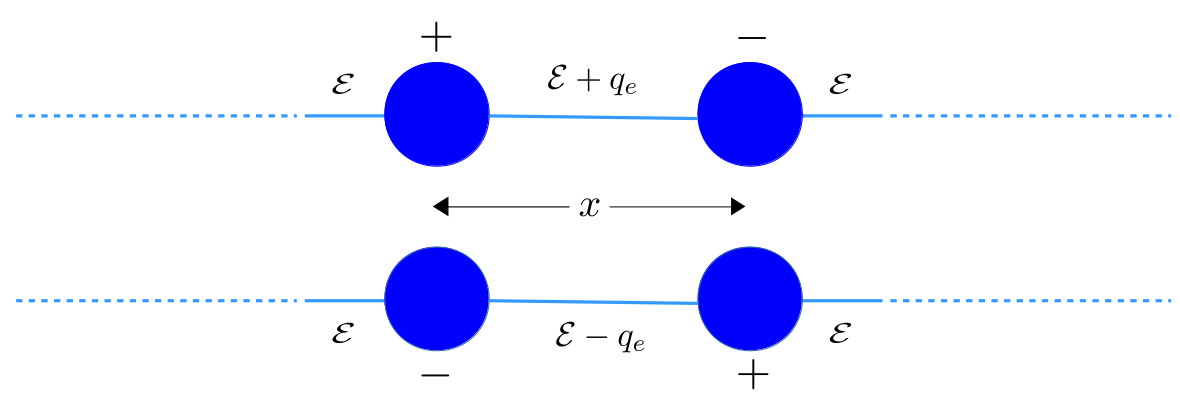
\includegraphics[scale=0.3]{figures/configuration.png}
	\caption{Two distinct configurations for particle-antiparticle pairs in one spatial dimension.}
	\label{fig:conf}
\end{figure}


The energy difference of this configuration compared to a vacuum state with no particles or antiparticles is given by 

\begin{equation}
\Delta E = \frac{1}{2}\int\dd{x}[(F_{01})² - \mathcal{E}²] = \frac{x}{2}[(\mathcal{E}\pm q_e)^2 - \mathcal{E}^2].\label{eq:energydiff}
\end{equation}

In essence, we can understand \eqref{eq:energydiff} as saying that it is energetically disfavorable for the vacuum to induce pair production if $|\mathcal{E}|\leq q_e/2$ . However, if $|\mathcal{E}|>q_e/2 $ the pair production from vacuum will set in and charges will travel to opposite edges of the spatial dimension until the field strength $\mathcal{E}$ is lowered below $q_e/2$.  This implies that the physics is periodic in $\mathcal{E}$ with period $q_e$.\\

Furthermore, we can define a dimensionless quantity  $$\mathcal{E}_0\overset{.}{=}\frac{\mathcal{E}}{q_e}$$ such that $\mathcal{E}_0\in[0,1]$. In the weak coupling limit $m/q_e\to\infty$, there is no particle-antiparticle pairs present and the vacuum energy density $\varepsilon$ is due to the electrostatic energy only since we can renormalize the Dirac sea energy of fermions to 0. Thus we have that in this limit

\begin{equation}
\varepsilon = 
\begin{dcases}
\frac{\mathcal{E}^2}{2} = \frac{q_e^2\mathcal{E}_0^2}{2}\quad \quad\quad\quad\quad\,\text{ if } \mathcal{E}_0\leq \frac{1}{2}& \\ \frac{(q_e-\mathcal{E})^2}{2} = \frac{q_e^2}{2}(1 - \mathcal{E}_0)^2\quad \text{ if } \mathcal{E}_0> \frac{1}{2}.
\end{dcases}
\end{equation}

\begin{figure}[htb]
	\centering
	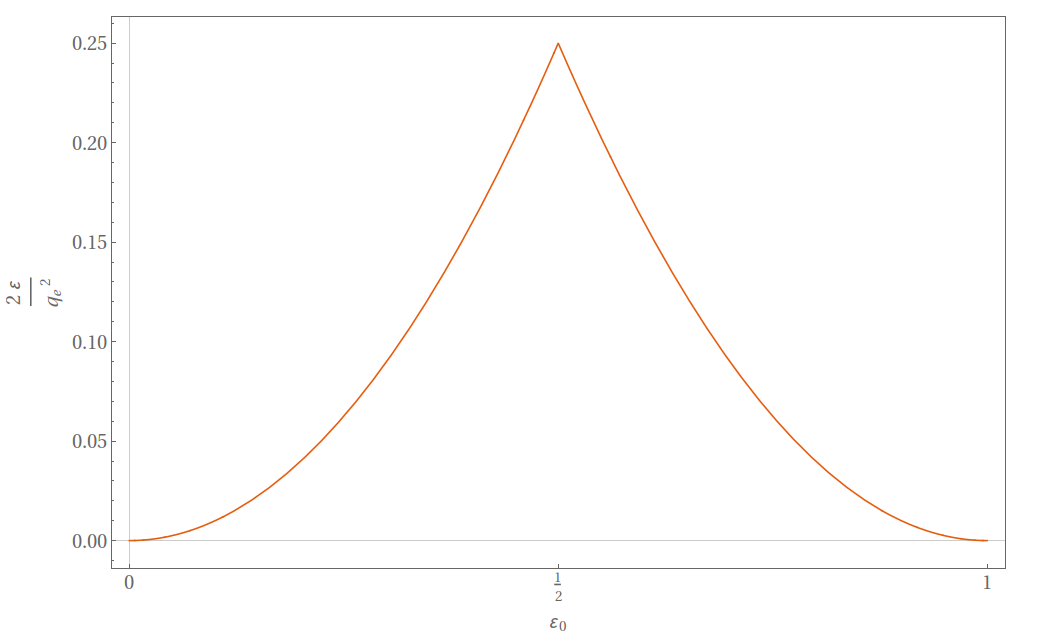
\includegraphics[scale=0.35]{figures/discont.png}
	\caption{Plot of energy density as a function of $\mathcal{E}_0$.}
	\label{fig:background}
\end{figure}

This is shown in figure  \ref{fig:background}. As we can see from figure \ref{fig:background}, $\varepsilon$ has a sharp peak at  $\mathcal{E}_0=1/2$, which points to the existence of a first order phase transition.


%---------SECTION--------%


\section{Chiral anomaly in the path integral formalism}\label{sec:ChiralAnomaly}

\subsection{Path integrals and the Grassman Jacobian}\label{ssec:PathIntegral}

Let us discuss the subtleties and important features of the Schwinger model that are closely related to the anomaly. Since the functional and path integral techniques are better suited to Euclidean space we will perform a Wick rotation $x_0 = -ix_4$ to arrive at Euclidean space with a negative metric $g_{\mu\nu} = -\delta_{\mu\nu}$. In Euclidean space we have that:

\begin{equation*}
    \partial_0 = i \partial_4,\quad A_0 =i A_4,\quad D_0 = iD_4,\quad\gamma^4 = i\gamma^0,\quad\gf=\gamma^0 \gamma^1 = i\gamma^1\gamma^4.
\end{equation*}
 
With this convention we have the following important relations in Euclidean space ($\mu = 4,1$):

\begin{equation}
    (\gmu)^\dagger = -\gmu
\end{equation}
\begin{equation}
    (\gmu)^2 = -1
\end{equation}
and
\begin{equation}
    (\gf)^2 = 1.
\end{equation}

Here the Dirac operator is Hermitian, $\slashed{D}^\dagger=\slashed{D}$ and $\varepsilon_{41} = i\varepsilon_{10}$. The following relations for the gamma matrices also hold in Euclidean space and will be useful throughout

\begin{equation}
    \gamma_\mu \gf = \edmn\gnu
\end{equation}

\begin{equation}
   \comm{\gmu}{\gnu} = -2\eumn\gf 
\end{equation}

\begin{equation}
    \Tr(\gmu \gnu) = \frac{1}{2} \Tr(\comm{\gmu}{\gnu} + \acomm{\gmu}{\gnu}) = -2\delta^{\mu\nu} 
\end{equation}

\begin{equation}
    \Tr(\gf \gmu \gnu) = 2 i \eumn.
\end{equation}

After this short detour on useful relations, let us explore the origin of the axial vector anomaly as a consequence of a change in the measure of the fermionic path integral. We start with the generating functional of a massless fermion $\psi$ coupled to electrodynamics in 2 dimensions

\begin{equation}
    \mathcal Z = \int \mathcal{D}A_\mu \mathcal{D}\psi \mathcal{D}\bar\psi e^{S[A,\psi,\bar\psi]}
\end{equation}

with the classical action 

\begin{equation}
    S = \int \dd[2]{x} \qty(\bar\psi (i\slashed{D})\psi - \frac{1}{4} F_{\mu\nu}^2).
\end{equation}

This theory has a $U_A(1)$ axial or chiral symmetry 

\begin{align}
    \psi\to e^{i\beta(x)\gf}\psi &= \psi + i \beta(x)\gf\psi\nonumber\\
    \bar\psi \to \bar\psi e^{i\beta(x)\gf} &= \bar\psi + i\bar\psi\beta(x)\gf
    \label{eq:chiraltrans}
\end{align}

with a corresponding Noether current $J_5^\mu$ for this symmetry. In quantum field theory, the classical Noether conservation law is replaced by the existence of Ward identities. To explore this we need to study the effect of the infinitesimal chiral transformation to the Grassmann integration measure $\mathcal{D}\psi \mathcal{D}\bar\psi$. First, we need to compute the functional Jacobian defined by

\begin{equation}
    \mathcal{D}\psi \mathcal{D}\bar\psi \to \mathcal{D}\psi' \mathcal{D}\bar\psi' = J[\beta]\mathcal{D}\psi \mathcal{D}\bar\psi.
\end{equation}

To first order in $\beta$ the fermionic Lagrangian changes like


\begin{align}
	\bar\psi' (i\slashed{D})\psi'&= (\psi + i \beta(x)\gf\psi)i\slashed{D}(\bar\psi + i\bar\psi\beta(x)\gf)\nonumber\\
	&= \bar\psi (i\slashed{D})\psi - [\partial_\mu\beta(x)]\bar\psi\gmu\gf\psi + \order{\beta^2}.
\end{align}

Therefore the fermionic part of the generating functional is transformed as follows

\begin{align}
	&\int \mathcal{D}\psi' \mathcal{D}\bar\psi' \exp\qty(\int \dd[2]{x}\bar\psi' (i\slashed{D})\psi)\nonumber \\
	&\to J[\beta]\int \mathcal{D}\psi \mathcal{D}\bar\psi \exp \qty(\int \dd[2]{x}\bar\psi(i\slashed{D} - \partial_\mu\beta(x) \gmu\gf)\psi)
	\label{eq:fermionicmeasure}
\end{align}

where both sides of \eqref{eq:fermionicmeasure} are Gaussian Grassmann integrals. These Gaussian integrals of Grassmann variables are equal to

\begin{equation}
\det(i\slashed{D}) = J[\beta]\det(i\slashed{D} - \partial_\mu\beta(x) \gmu\gf ),
\end{equation}

thus the value of the Jacobian $J[\beta]$ is given as the ratio of two determinants.\\

Now, we need to expand the spinors in terms of eigenfunctions of the Dirac operator

\begin{equation}
i\slashed{D}\phi_n \equiv i(\slashed{\partial} + ie\slashed{A})\phi_n = \lambda_n \phi_n,
\end{equation}

having the completeness relation given by the inner product

\begin{equation}
\int \dd[2]{x} \phi_n^\dagger(x) \phi_m(x) = \delta_{nm}.
\end{equation}

Thus, on this basis the spinors are decomposed as

\begin{equation}
\psi = \sum_n a_n \phi_n ;\quad \bar\psi = \sum_n b_n \phi_n^\dagger,
\label{eq:spinorexpansion}
\end{equation}

where the coefficients $a_n$ and $\bar b_n$ are independent elements of the Grassmann algebra. The fermionic measure is then defined to be 

\begin{equation}
\mathcal{D}\psi\mathcal{D}\bar\psi \overset{.}{=}\prod_{n}\dd b_n\dd a_n.
\end{equation}

Under a chiral transformation \eqref{eq:chiraltrans} the Grassmann coefficients in \eqref{eq:spinorexpansion} are transformed to

\begin{equation}
\psi = \sum_n a_n' \phi_n = \sum_n a_n e^{i\beta(x)\gf }\phi_n
\end{equation}

which implies that infinitesimally

\begin{align}
	a_n' &= \sum_n \int \dd[2]{x}\phi_m^\dagger(x)(1 + i\beta(x)\gf + \ldots)\phi_n(x) a_n\nonumber\\
	&= \sum_n\qty(\delta_{nm} + \mathbb{A}_{nm})a_n.
\end{align}

Therefore, the measure is transformed as

\begin{equation}
\prod_n \dd a'_n = [\det\qty(1+\mathbb{A}_{nm})]^{-1} \prod_n \dd a_n,
\label{eq:invdet}
\end{equation}
the inverse power of the determinant is a consequence of the translation invariance of the Grassmann integration measure and the fact that Grassmann integration is the same as usual differentiation with the equivalence given by $$\dd a_n \equiv \pdv*{}{a_n}.$$ The Jacobian for $\mathcal{D}\bar\psi$ gives rise to an identical factor as \eqref{eq:invdet}. Consequently, we have that

\begin{equation}
    \prod_{n}\dd b_n\dd a_n. = [\det\qty(1+\mathbb{A}_{nm})]^{-2} \prod_n \dd b_n \dd a_n,
\end{equation}

Thus, we need to compute $$\det\qty(1+\mathbb{A}_{nm}) = \exp\qty({\tr\log(1+\mathbb{A}_{nm})}),$$ which to first order in $\beta$ is simply $\exp(\tr\mathbb{A}_{nm})$. Hence,

\begin{equation}
    J[\beta] = [\det\qty(1+\mathbb{A}_{nm})]^{-2} = \exp\qty(-2i\int \dd[2]{x}\beta(x)\sum_n \phi_n^\dagger(x) \gf \phi_n(x)).
    \label{eq:determinant}
\end{equation}

\subsection{Dirac operator mode regularization}

The coefficient of $\beta(x)$ is $\tr\gf$ which is zero. However, the trace is also over an infinite number of eigenstates of $i\slashed{D}$, which of course is infinite. Consequently, \eqref{eq:determinant} is an ill-defined sum which should be regularized in order to obtain a sensible result. We can regulate \eqref{eq:determinant} by introducing a UV-regulator to cut off the sum at large eigenvalues

\begin{equation}
    \sum_n \phi_n^\dagger(x) \gf \phi_n(x) \equiv \lim_{M\to\infty} \sum_n \phi_n^\dagger(x)\gf \phi_n(x)e^{\lambda_n/M^2}.
    \label{eq:regularized}
\end{equation}

Since the $\phi_n$ are eigenfucntions of $i\slashed{D}$ we can introduce the one-particle Hilbert space $\{\ket{x}\}$ and write \eqref{eq:regularized} equivalently as

\begin{equation}
    \lim_{M\to\infty} \sum_n \phi_n^\dagger(x)\gf e^{(i\slashed{D})^2/M^2}\phi_n(x)=\lim_{M\to\infty}
     \ev**{\tr\qty(\gf e^{(i\slashed{D})^2/M^2})}{x}.
\end{equation}

This being so, we need to find an expression for $-\slashed{D}^2$ in terms of the gauge field $A_\mu$. This is done as follows, consider the Dirac equation

\begin{equation}
    i(\slashed{\partial} + iq_e\slashed{A})\psi = 0,
\end{equation}

since it is equated to zero we can multiply it by whatever we want. An intelligent choice is to multiply by

\begin{align}
        0&=(i\slashed{\partial} - q_e\slashed{A})(i\slashed{\partial} - q_e\slashed{A})\psi\nonumber\\
        &= \qty(\frac{1}{4}\acomm{i\partial_\mu - q_eA_\mu}{i\partial_\nu - q_eA_\nu}\acomm{\gmu}{\gnu}+ \comm{i\partial_\mu - q_eA_\mu}{i\partial_\nu-q_eA_\nu}\comm{\gmu}{\gnu})\psi\nonumber\\
        &= \qty[ (i\partial_\mu - q_eA_\mu)(i\partial_\nu - q_eA_\nu) g^{\mu\nu} + \frac{iq_e}{2} F_{\mu\nu}\eumn\gf]\psi\nonumber\\
        &= \qty[(i\partial_\mu - q_eA_\mu)^2 +\frac{iq_e}{2} F_{\mu\nu}\eumn\gf]\psi.
        \label{eq:diracsq}
\end{align}

We recognize the expression inside brackets as $\slashed{D}^2 = D^2 + \frac{iq_e}{2} F_{\mu\nu}\eumn\gf$. 

Moreover, we need to evaluate

\begin{align}
    \lim_{M\to\infty}\beta(x)\ev**{\tr\qty(\gf \exp(-\frac{(\partial-q_eA)^2 + \frac{iq_e}{2} F_{\mu\nu}\eumn\gf }{M^2}))}{x}
\end{align}

Expanding the exponential to extract the contribution to leading $e$ we get that

\begin{equation}
    \lim_{M\to\infty}\beta(x)\ev**{\tr\qty(\gf \exp(-\frac{(\partial-q_eA)^2}{M^2})\qty(1 - \frac{iq_e}{2} F_{\mu\nu}\eumn\gf))}{x}.
\end{equation}

Here we can set $A=0$ obtaining

\begin{align}
        &\lim_{M\to\infty}\beta(x)\ev**{\tr\qty(\gf e^{-\frac{\partial^2}{M^2}}\qty(1 - \frac{iq_e}{2} F_{\mu\nu}\eumn\gf))}{x} \nonumber\\ &=\lim_{M\to\infty}\beta(x)\qty(\frac{-iq_e}{2M^2}F_{\mu\nu}\eumn)\tr[(\gf)^2] \ev**{e^{-\frac{\partial^2}{M^2}}}{x}.
\end{align}

Using the fact that

\begin{equation}
\ev**{e^{-\frac{\partial^2}{M^2}}}{x} = i\int \frac{\dd[2]{k_E}}{(2\pi)^2}e^{-k_E/M^2}=\frac{i M^2}{2\pi},
\end{equation}

where the subscript $E$ refers to Euclidean momenta. We have that the contribution to leading order in $e$ is independent of $M$. Hence, when the regulator mass $M\to\infty$ we obtain

\begin{equation}
\frac{q_e}{4\pi}F_{\mu\nu}\eumn.
\end{equation}
which is the 2 dimensional version of the Adler–Bell–Jackiw anomaly \cite{Bell1969,Adler}.\\

Hence, the evaluation of the Jacobian $J[\beta]$ in \eqref{eq:determinant} is

\begin{equation}
J[\beta] = \exp\qty(i \int\dd[2]{x}\beta(x)\frac{q_e}{2\pi}F_{\mu\nu}\eumn).
\end{equation}

The result of a chiral transformation to the fermionic measure is then

\begin{multline}
           \int \mathcal{D}\psi \mathcal{D}\bar\psi \exp\qty(\int \dd[2]{x}\mathscr{L}_{\text{QED}_2})\\
        \to \int \mathcal{D}\psi \mathcal{D}\bar\psi \exp \qty(\int \dd[2]{x}\mathscr{L}_{\text{QED}_2} -J^5_\mu \partial_\mu \beta(x) +i\beta(x)\frac{q_e}{2\pi}F_{\mu\nu}\eumn )
        \label{eq:intanomaly}
\end{multline}



\subsection{Schwinger-Dyson equation for a gauge symmetry}\label{ssec:SchwingerDyson}

In classical field theory, Noether's theorem stems from the fact that a variation of the field being a global symmetry of the Lagrangian leads to the existence of a classical conserved Noether current. The quantum field theory counterpart of this procedure, in the path integral formalism, will produce a powerful result concerning the correlation functions the theory. To derive the result let us consider the correlation function of $\psi(x_1)$ and $\bar\psi(x_2)$ in a fermionic theory with a \emph{global symmetry} $$\psi\to e^{i\alpha}\psi,$$
this correlator reads

\begin{equation}
    \expval{\psi(x_1)\bar\psi(x_2)} = \int \mathcal{D}\psi \mathcal{D}\bar\psi \exp\qty(\int \dd[2]{x}\bar\psi(i\slashed{\partial} + m)\psi)\psi(x_1)\bar\psi(x_2).
\end{equation}

The field transform locally as

\begin{equation}
    \psi(x)\to e^{-i\alpha(x)}\psi(x);\quad  \bar\psi(x)\to e^{i\alpha(x)}\bar\psi(x)
    \label{eq:transformation}
\end{equation}

Therefore, under this transformation, the Lagrangian is not invariant, as it acquires the following terms

\begin{equation}
    i\bar\psi\slashed{\partial}\psi \to i\bar\psi\slashed{\partial}\psi + \bar\psi\gmu\psi\partial_\mu\alpha(x),
\end{equation}

and

\begin{equation}
    \psi(x_1)\bar\psi(x_2)\to e^{-i\alpha(x_1)}e^{i\alpha(x_2)}\psi(x_1)\bar\psi(x_2)
\end{equation}

The path integral is invariant under \emph{any} field redefinition up to a Jacobian factor, $J[\alpha]$, which in the case of a transformation like \eqref{eq:transformation} is equal to 1. Hence, expanding to first order in $\alpha$ leads to the following relation

\begin{align}
    0 = &\int \mathcal{D}\psi \mathcal{D}\bar\psi e^{i S[\psi,\bar\psi]}\qty(i \int \dd[2]{x}\bar\psi\gmu\psi\partial_\mu\alpha(x))\psi(x_1)\bar\psi(x_2)\nonumber\\
    &+ \int \mathcal{D}\psi \mathcal{D}\bar\psi e^{i S[\psi,\bar\psi]}\qty(-i\alpha(x_1)\psi(x_1)\bar\psi(x_2) + i\alpha(x_2) \psi(x_1)\bar\psi(x_2)).
\end{align}

A simple and clever rearrangement of the previous relation yields the following very important result:

\begin{align}
    &\int \dd[2]{x}i \alpha(x)\partial_\mu \int \mathcal{D}\psi \mathcal{D}\bar\psi e^{i S[\psi,\bar\psi]}\qty(\bar\psi\gmu\psi)\psi(x_1)\bar\psi(x_2)\nonumber\\
    &= \int \dd[2]{x}i \alpha(x) \qty(\delta(x-x_2) - \delta(x-x_1))\int \mathcal{D}\psi \mathcal{D}\bar\psi e^{i S[\psi,\bar\psi]}\psi(x_1)\bar\psi(x_2).
\end{align}

Since this must hold for arbitrary $\alpha$, we have the following relation for the correlation functions

\begin{equation}
\partial_\mu \expval{J^\mu\psi(x_1)\bar\psi(x_2)} = -\delta(x-x_1)\expval{\psi(x_1)\bar\psi(x_2)} + \delta(x-x_2)\expval{\psi(x_1)\bar\psi(x_2)}
\end{equation}

where we have recalled the definition of the U(1) electromagnetic current $J^\mu \overset{.}{=}\bar\psi\gmu\psi$. This relation is the quantum conservation law analogous to the classical $\partial_\mu J^\mu = 0$ and holds for time-ordered correlation functions in quantum field theory. Moreover, the relation is easily generalized to higher order correlation functions. It contains one delta function for each spinor field $ \psi_i$ of charge $Q_i$ in the correlation function \cite{Schwartz}, namely

\begin{multline}
   \partial_\mu \expval{J^\mu\psi(x_1)\bar\psi(x_2)A^\nu(x_3)\bar\psi(x_4)+\cdots} =\\
    \sum Q_i \delta(x-x_i)\expval{\psi(x_1)\bar\psi(x_2)A^\nu(x_3)\bar\psi(x_4)+\cdots}
\end{multline}

This equation is independent of gauge fixing and thus neither the photon field $A^\nu$ nor the photon kinetic term $F^{\mu\nu}$ have any effect in the final expression for the correlation function.\\

Hence, in the case of \eqref{eq:intanomaly} the proper relation for the correlator function reads


\begin{equation}
    \partial_\mu \expval{J_5^\mu \,\mathcal{O}(x_1\ldots x_n)} = [i]\frac{q_e}{2\pi}\expval{\eumn F_{\mu\nu}\, \mathcal{O}(x_1\ldots x_n)}
    \label{eq:anomalousdiv}
\end{equation}

for any local operator $\mathcal{O}(x_1\ldots x_n)$. It is important to note that the factor $i$ in brackets in front of the result is absent in Minkowski space. In such a way and after a rather long calculation, we have found that the anomalous divergence of the axial current in the Schwinger model which is given by \eqref{eq:anomalousdiv}.


%---------SECTION--------%


\section{Anomaly, index and topology}\label{sec:topology}

\subsection{Zero-modes and index of the Dirac operator}\label{ssec:ZeroModesIndex}

Fujikawa realized that the exponential in the transformation of the Jacobian $J[\beta]$ represents an \emph{``index density''} of the Dirac operator \cite{Fujikawa1980}. To see this let us introduce the following projectors

\begin{equation}
    P_{\pm} = \frac{1\pm\gf}{2},
\end{equation}

such that

\begin{equation}
    P_\pm  \psi = \psi_{\pm};\quad \gf\psi_{\pm} = \pm \psi_{\pm},
\end{equation}

with the positive and negative chirality spinors

\begin{equation}
    \psi_-= \mqty(\psi_1  \\ 0), \quad \psi_+ = \mqty( 0 \\ \psi_2).\label{eq:spinorchiral}
\end{equation}

Let us recall that we can expand the Dirac operator in eigenmodes:

\begin{equation}
    i\slashed{D}\psi_n  = \lambda_n \psi_n,
\end{equation}

since $\acomm{\gmu}{\gf}=0$, $\gf\psi_n$ satisfies the following eigenvalue equation 

\begin{equation}
     i\slashed{D}\gf\psi_n = - \lambda_n \gf\psi_n.
\end{equation}

Now, given the inner product in Euclidean space and using the fact that $i\slashed{D}$ is Hermitian, for $\lambda_n\neq 0$ we have hat both eigenfunctions are orthogonal, viz

\begin{equation}
    \braket{\psi_n}{\gf\psi_n} = \int \dd[2]{x} \psi_n^*(x) \gf\psi_n(x) =0.
\end{equation}

Nonetheless, for $\lambda_n = 0$, we can define \emph{zero-modes} $\Phi_n$ which satisfy

\begin{equation}
     i\slashed{D}\Phi_n = 0;\quad i\slashed{D}\gf\Phi_n = 0,
\end{equation}

being simultaneously eigenfunctions of $\gf$ for positive and negative chirality spinors

\begin{equation}
    \gf \Phi_{n}^+ = + \Phi_{n}^+;\quad \gf \Phi_{n}^- = + \Phi_{n}^-.
\end{equation}

Recalling the transformation of the Jacobian $J[\beta]$ in terms of the eigenmodes of the Dirac operator  \eqref{eq:determinant}, we obtain, in terms of the zero-modes

\begin{align}
    \int \dd[2]{x} \sum_n \psi_n^* \gf \psi_n &= \int\dd[2]{x} \sum_{\substack{n \\ \lambda_n=0}}\Phi_n^{+*}\gf \Phi_n \nonumber\\
    &=  \sum_{\substack{n \\ \lambda_n=0}} \int\dd[2]{x}\Phi_n^{+*} \Phi_n^+ - \sum_{\substack{n \\ \lambda_n=0}}\int\dd[2]{x}\Phi_n^{-*} \Phi_n^- \equiv (n_+ - n_-).
    \label{eq:zeroIndex}
\end{align}

Here we see the appearance of the number of zero-modes of positive and negative chirality, respectively $n_+$ and $n_-$. The difference in equation \eqref{eq:zeroIndex} is known as the \emph{index} of a differential operator. The differential operator we are considering is

\begin{equation}
    D_+ \equiv  i\slashed{D}P_+
\end{equation}

with the adjoint operator given by

\begin{equation}
     D_+^\dagger = D_- \equiv  i\slashed{D}P_-.
\end{equation}

These operators act on the subspaces of positive and negative chirality respectively. Now, the index of a Fredholm operator such as $D_+$ is defined as

\begin{equation}
\text{ind}D_+= \dim(\ker D_+) - \dim(\text{coker}D_+) = \dim(\ker D_+) - \dim(\ker D_+^\dagger),
\label{eq:index}
\end{equation}

but the difference in \eqref{eq:index} is precisely $n_+ - n_-$, the difference between the number of positive and negative chirality zero-modes.\\

To make a connection to the anomaly computation done in section \ref{sec:ChiralAnomaly} let us recall that in order to make sense of the Jacobian $J[\beta]$, we had to include an UV-regulator. This regulator allowed us to compute the sum in equation \eqref{eq:zeroIndex} in terms of the gauge field strength tensor. Combining \eqref{eq:zeroIndex} and \eqref{eq:regularized} yields

\begin{equation}
\frac{q_e}{4\pi}\int\dd[2]{x}\edmn F^{\mu\nu} = (n_+ - n_-)\equiv \text{ind} D_+.
\end{equation}

This result is the \emph{Atiyah-Singer theorem} for the Dirac operator coupled to a $U(1)$ gauge field in two-dimensional Euclidean space.


\subsection{Atiyah-Singer index theorem}\label{ssec:Atiyah}

Atiyah and Singer \cite{Atiyah1963} showed that the index of an elliptic differential operator can be expressed in terms of purely topological quantities. In the case of the Dirac operator coupled to a Yang-Mills field in even-dimensional space their result is

\begin{equation}
\text{ind}D_+ = \int_{\mathcal{M}}\text{ch}F
\end{equation}

where $\text{ch}$ is the Chern character and $\mathcal{M}$ is a compact $2n$-dimensional manifold equipped with a spin connection $\omega$. The Chern class is given by

\begin{equation}
\text{ch}F = \tr e^{\frac{i}{2\pi}F} = \pmb r + \frac{1}{2\pi}\tr F + \frac{1}{2!}\qty(\frac{i}{2 \pi})\tr F^2 + \ldots
\label{eq:chern}
\end{equation}

for a representation $\pmb r$ of a $SU(N)$ (or $U(N)$) gauge connection $A$, with curvature 2-form $F=\dd A + A^2$. Since the integral is done over $\mathcal{M}$ only the $n$-th term in
\eqref{eq:chern} survives. Moreover since all physical quantities vanish at infinity, in particular $J_\mu^5 \overset{\infty}{\longrightarrow} 0$, we can compactify $\mathbb{R}^2$ onto the unit sphere $S^2$ and perform the integration with $\mathcal{M}=S^2$. This is equivalent to solving the integral with $\mathcal{M}=\mathbb{R}^2$ and dropping the surface term at infinity by using the anomalous divergence of $J_\mu^5$ (cf. section 4.7.2 in \cite{abdalla}), thus

\begin{equation}
\text{ind}D_+ = \frac{q_e}{2\pi}\int_{S^2}\frac{1}{2} F_{\mu\nu}\dd x^\mu \dd x^\nu = \frac{q_e}{4\pi}\int_{S^2} {}^\ast F \edmn \dd x^\mu \dd x^\nu = \frac{q_e}{4\pi}\int\dd[2]{x}\eumn F_{\mu\nu},
\end{equation}

which is in consonance with Fujikawa's computation of the chiral anomaly. Thus, we can employ a topological result to compute the chiral anomaly associated with this U(1) gauge theory.


%---------SECTION--------%


\section{Anomaly and the fermion spectrum}\label{sec:FermionSpectrum}

\subsection{Schwinger model on a circle}\label{ssec:SchCircle}

Let us consider a system with a Lagrangian given by \eqref{eq:lagrangian} on a one-dimensional universe of length $L$ compactified into a circle $S^1$. We can impose periodic boundary conditions on the $A_\mu$ field and antiperiodic boundary conditions to the fermions $\psi$

\begin{align}
	A_\mu(t,x=-L/2) = A_\mu(t,x=L/2)\nonumber\\
	\psi(t,x=-L/2) = - \psi(t,x=-L/2)\label{eq:BC}.
\end{align}

Moreover, we can work in a gauge where $A_0=0$ and choose $A_1(t)$ as an \emph{external field} which can be treated as an adiabatic perturbation to the system. As a consequence of the gauge freedom 

\begin{equation*}
	A_\mu \to A_\mu + \partial_\mu \Lambda(x,t), \quad \psi \to e^{i\Lambda(t,x)}\psi
\end{equation*}

The gauge transformation $\Lambda(x,t)$ can be chosen to be
\begin{equation}
\Lambda(x,t) = \frac{2\pi}{L} nx;\quad n=\pm1,\pm2,\ldots
\end{equation}

which is in accordance with the boundary conditions imposed in \eqref{eq:BC} since $\partial_x\Lambda(x,t) = \text{const}$ and $\partial_t\Lambda(x,t) = 0 $. Which means that neither the periodic nature of $A_1$ nor the anti-periodic nature of $\psi$ are violated by the gauge function, since the phase factor at $-L/2$ and $L/2$ is a multiple of $2\pi n$. As a result of this, the physically meaningful values of $A_1$ are restricted to the interval $[0,2\pi/L]$, since values outside this interval are gauge equivalent to a point inside the interval. This implies that the gauge field $A_1$ lives in a circle of length $2\pi/L$ where it takes physical values. \\

The Lagrangian of the theory is invariant under a $U(1)$ symmetry 

\begin{align}
    \psi\to e^{i\Lambda(x)}\psi \nonumber\\
    \bar\psi \to \bar\psi e^{-i\Lambda(x)}
\end{align}

which gives rise to the conservation of electric charge and vector current

\begin{equation}
    \partial_\mu J^\mu = 0,\quad \dot{Q}(t) = 0
\end{equation}

with
\begin{equation}
    Q(t) = \int \dd{x} J_0(t,x)\label{eq:q}.
\end{equation}

Additionally it has an axial symmetry $U_A(1)$ 
\begin{align}
    \psi\to e^{i\beta(x)\gf}\psi\nonumber\\
    \bar\psi \to \bar\psi e^{i\beta(x)\gf}
\end{align}

which yields the conservation of the axial current and the axial charge

\begin{equation}
    \partial_\mu J_5^\mu = 0,\quad \dot{Q_5}(t) = 0
\end{equation}

with

\begin{equation}
    Q(t) = \int \dd{x} J^5_0(t,x).\label{eq:q5}
\end{equation}

Classically both $Q(t)$ and $Q_5(t)$ are conserved.\\

Recalling the decomposition of the spinor in positive and negative chiralities \eqref{eq:spinorchiral} then the axial charge of the positive chirality spinor is $Q_5^+ = +1$ and the one for the negative chirality spinor is $Q_5^+ = -1$. Therefore, the conservation of both $Q$ and $Q_5$ implies the \emph{classical} conservation of the number of the positive and negative chirality particles separately. However, quantum mechanically both \eqref{eq:q} and \eqref{eq:q5} cannot be conserved simultaneously as a consequence of the \emph{chiral anomaly} and only $Q(t)$ is conserved after quantization.


In 1+1 dimensional QED, choosing a representation of the gamma matrices as \eqref{eq:gammarep1}, the Dirac equation is written as

\begin{equation*}
	[i (\gamma^0 \partial_t + \gamma^1 \partial_x) + q_e (\gamma^0 A_0 + \gamma^1 A_1)]\psi = 0 
\end{equation*}

which reduces to (recalling we have set $A_0=0$) 

\begin{equation}
\partial_t \psi =- \sigma_3(i \partial_x - q_e A_1)\psi  \label{eq:scheq}.
\end{equation}

Due to the form of \eqref{eq:scheq} and the boundary conditions \eqref{eq:BC} we can use a Fourier expansion of the spinors 

\begin{equation}\label{eq:fourierSpinor}
\psi(t,x) = \frac{1}{\sqrt{L}} \sum_k u(k) e^{-iE_kt}\exp\qty[i\qty(k + \frac{1}{2})\frac{2\pi}{L} x],\quad k\in\mathbb{Z} 
\end{equation}

which satisfies the following ``stationary Schrödinger'' equation

\begin{equation}
E_k \psi_k(x) = -\sigma_3 (i\partial_x - q_e A_1)\psi_k(x).
\end{equation}

We can see that the energies for the $k$-th level of the positive and chirality spinors are respectively

\begin{align}
E_k^- = \frac{2\pi}{L}\qty(k + \frac{1}{2}) + q_e A_1\label{eq:energy+}\\
E_k^+ = -\frac{2\pi}{L}\qty(k + \frac{1}{2}) - q_e A_1\label{eq:energy-}.
\end{align}

\begin{figure}[htb]
    \centering
    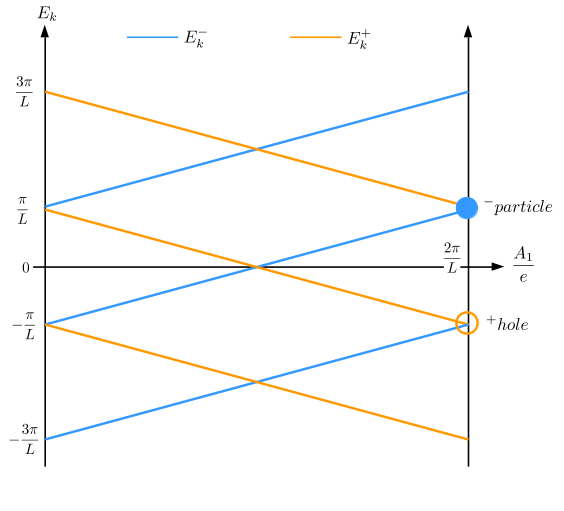
\includegraphics[scale=0.5]{figures/spectrum.png}
    \caption{Fermion spectrum as function of $A_1$.}
    \label{fig:spectrum}
\end{figure}

The spectrum is plotted in figure \ref{fig:spectrum}. We can see that the spectrum has a linear dependence on $A_1$. At $A_1=0$ the energy levels of the positive and negative chirality fermions are degenerate. However, as $A_1$ increases the energy levels split. At $A_1=2\pi/L$ the degeneracy occurs again as expected since this point is gauge equivalent to $A_1=0$. Moreover, the restructuring of the spectrum when $A_1$ changes from $0$ to $2\pi/L$ is non-trivial since the positive chirality levels are shifted downwards while the negative chirality levels are shifted upwards. This restructuring of the spectrum is the essence of the chiral anomaly.

\subsection{Infrared and ultraviolet behavior}\label{ssec:SpectrumIR}

Let us now construct the ground state of the theory following Dirac's prescription of filling the Dirac sea while leaving all the positive energy levels empty. This can easily be done by looking at figure \ref{fig:spectrum}, viz

\begin{equation}
    \ket{\psi_\text{vac}} = \qty[\prod_{k=-1,-2,\ldots}\ket{1_k}_-]\qty[\prod_{k=0,1,2,\ldots}\ket{1_k}_+]
    \label{eq:gsk}
\end{equation}

where the 1 denotes either a positive or negative chirality level filled having momentum k as given, by \eqref{eq:fourierSpinor}. At $A_1=0$, by construction, we have a vacuum state of the fermions. Nevertheless, by increasing $A_1$ to $2\pi/L$ we produce, by the restructuring of the spectrum, a $^-$particle and a $^+$hole (represented by circles in figure \ref{fig:spectrum}). This energy level restructuring implies a net change in the conserved charges. The appearance of both a particle and a hole does not change the electric charge $Q$ since the particle and the hole carry opposite electric charges. Nonetheless, the axial charges of the particle and the hole are identical ($Q_5=1$) and thus the restructuring of the spectrum induces a net change in $Q_5$ given by

\begin{equation}
\Delta Q_5 = 2 \label{eq:q5change}.
\end{equation}

This can be rewritten in terms of $A_1$ as

\begin{equation}
\Delta Q_5 = \frac{q_e L}{\pi}\Delta A_1,
\end{equation}

we can divide it by $\Delta t$  getting the following time evolution equation

\begin{equation}
\dot{Q_5} = \frac{q_e L}{\pi}\dot{A_1}
\end{equation}

which written as the conserved quantity is

\begin{equation}
\frac{\partial}{\partial t} \int \dd{x}\qty(J^5_0(x,t) - \frac{q_e}{\pi}A_1) = 0.
\end{equation}

The current is given by

\begin{equation}
\bar{J}_\mu^5  = J_\mu^5 - \frac{q_e}{\pi}\eumn A_\nu;\quad \partial^\mu\bar{J}_\mu^5=0
\end{equation}

we have recovered the usual chiral anomaly result derived in section \ref{sec:ChiralAnomaly}

\begin{equation}
\partial^\mu J_\mu^5 = \frac{q_e}{2\pi}\edmn \partial^\mu A^\nu.
\label{eq:anomaly2}
\end{equation}

Therefore, in this context, the anomaly presents as a result of the crossing of the energy levels at the energy $E=0$ as a consequence of a variation of the value of the gauge filed $A_1$. This analysis is known as an \emph{infrared} argument since it pertains low energies.\\

However, we can also study the anomalous behavior by introducing an \emph{ultraviolet cutoff} to regularize the theory at high energy scales. The vacuum wavefunction being a superposition of infinitely many filled states of the Dirac sea is a divergent quantity. To obtain a sensible result, we have to introduce a gauge invariant regulator. A first naive idea for regularization is to impose a limit on the number of modes such that $k\in[-k_{\text{max}},k_{\text{max}}]$, however, this type of regularization breaks gauge invariance and electric charge conservation. A regularization procedure that preserves gauge invariance is the gauge invariant point-splitting method due to Schwinger \cite{Sch1951}. In this scheme, we can introduce the regularized currents that avoid the divergences of the form

\begin{align}
    J^\mu_{\text{reg}} &= \lim_{\epsilon\to 0} \bar{\psi}(t,x+\epsilon)\gmu \psi(t,x)\exp\qty(i q_e \int_x^{x+\epsilon}\dd{x}A_1),\nonumber\\
    J^\mu_{5\text{ reg}} &= \lim_{\epsilon\to 0} \bar{\psi}(t,x+\epsilon)\gmu\gf \psi(t,x)\exp\qty(i q_e \int_x^{x+\epsilon}\dd{x}A_1)\label{eq:pointSplitting}
\end{align}

The new regularized charges are therefore defined to be

\begin{align}
    &Q^{\text{reg}} (t)= \int \dd{x}J^{\text{reg}}_0 (t,x)\nonumber\\
    &Q_5^{\text{reg}} (t) = \int \dd{x}J^{\text{reg}}_{0\,5} (t,x),
\end{align}

and for the charges of the positive and negative chirality spinors

\begin{align}
    Q_- = \frac{Q - Q_5}{2}\nonumber\\
    Q_+ = \frac{Q + Q_5}{2}.
\end{align}

Using the regularized current expression \eqref{eq:pointSplitting} and the Fourier expansion of the spinors, we can calculate the positive and negative chirality charges explicitly yielding the following sums over $k$

\begin{align}
    Q_- = \sum_{k=-1}^{-\infty} \exp\qty(-i \epsilon\qty[\qty(k + \frac{1}{2})\frac{2\pi}{L} - q_e A_1])\nonumber\\
    Q_+ = \sum_{k=0}^{\infty} \exp\qty(-i \epsilon\qty[\qty(k + \frac{1}{2})\frac{2\pi}{L} - q_e A_1]).
\end{align}

The summations for $Q_+$ and $Q_-$  run over a different sets of $k$'s as one can see from figure \ref{fig:spectrum} and from equation \eqref{eq:gsk}. The negative chirality Dirac sea is field with modes $k=-1,-2,\ldots$, while the positive chirality Dirac sea is filled with modes $k=0,1,2,\ldots$. Doing the summation and the expanding in $\epsilon$ we can study the divergent part of both $Q_-$ and $Q_+$, viz

\begin{align}
    &Q_-=-\frac{ L}{2\pi}\frac{1}{i\epsilon} + \frac{q_e L}{2\pi}A_1 + \order{\epsilon}\nonumber\\
    &Q_+ = \frac{ L}{2\pi}\frac{1}{i\epsilon} - \frac{q_e L}{2\pi}A_1 + \order{\epsilon}.\label{eq:chargesUV}  
\end{align}
 
The physical charges of the theory are $Q$ and $Q_5$. These are defined  in terms of $Q_-$ and $Q_+$ as

\begin{equation}
Q = Q_- + Q_+;\quad Q_5 = Q_+ - Q_-
\end{equation}

hence, by using result \eqref{eq:chargesUV} we find that in fact, the electric charge $Q$ is conserved

\begin{equation}
\Delta Q = 0.
\end{equation}

Nevertheless, the chiral charge $Q_5$ has a net change of

\begin{equation}
\Delta Q_5 = 2\frac{L}{2\pi}A_1.
\end{equation}

Whenever the value of $A_1$ varies from $0$ up to $2\pi/L$, this is consistent with the result already presented in subsection \ref{ssec:SpectrumIR}.\\
 
 This analysis suggests to us a different interpretation of the chiral anomaly in the Schwinger model. Previously, the anomaly presented itself as a non-conservation of the chiral charge due to the fermion spectrum restructuring. The energy levels of fermions and anti-fermions cross the zero point energy of the vacuum creating a net excess of chiral charge. Nevertheless, by analyzing the ultraviolet behavior of the model we can note that the chiral charge non-conservation is a consequence of the energy levels crossing the ultraviolet cut-off $\epsilon$ we imposed to regularize the physically relevant quantities. Note that both the crossing of the levels at the vacuum energy and the departure beyond the ultraviolet cut-off are simultaneous processes. Hence, both the infrared and ultraviolet analyses are adequate to explain the physics of the anomaly as a dynamic restructuring of the energy level of the Dirac spectrum.
 
 %---NEW---%
 
 \section{Comments and conclusion}\label{sec:Conclusion1}
 
  Throughout this chapter, we have studied various important physical aspects of quantum electrodynamics in (1+1)-dimensions, i.e. the Schwinger model. In the first section \ref{sec:LagrangianHamiltonian} we derived the equations of motion of the theory which are the \emph{Dirac equation} and \emph{Maxwell's equations}, also we computed the \emph{Hamiltonian} of the theory, which will be very important later on within this thesis. Using the equations of motion, the simplicity of electrodynamics in one spatial dimension, and the anomalous divergence of the axial Noether current we showed that the theory has a massive "photon" whose mass is given in terms of the electromagnetic coupling constant, viz
 
 \begin{equation*}
 	m_\gamma =\frac{q_e}{\sqrt{\pi}}.
 \end{equation*}
 
 Let us stop for a moment and comment on the relevance of this. We started with QED in (1+1)-dimensions, where the photon is massless as it is expected from Maxwell's equations. Nevertheless, we found that as a consequence of the chiral anomaly of the model, resulting from the $U_A(1)$ symmetry associated to the chirality of the fermions the photon has acquired a non-zero mass. Therefore, the incompatibility of chiral symmetry with the quantization of the theory, i.e. the chiral anomaly, has generated a Higgs-like mechanism of "dynamic" mass generation  (dynamic since it is realized at the level of the equations of motion) for the photon, where its mass follows immediately from breaking of the classical axial symmetry. Furthermore, this can also be understood as a result of the Coulomb's potential being linear with the distance $\pmb{r}$ between the charges in $D=2$, which makes the theory a \emph{confining} one, much like QCD$_4$. Thus, we can make the "heuristic" argument (since a formal argument would be outside the scope of this thesis) that the theory develops a mass gap. In fact, the theory is equivalent of a free massive scalar particle of mass $m_\gamma$ where this massive particle is interpreted as a bound state of a fermion anti-fermion pair \cite{Lowenstein1971}.\\
 
 Additionally, in subsection \ref{ssec:BackgroundField} we explored how in one spatial dimension the presence of a background electric field $\mathcal{E}$ induces vacuum pair production which due to the energetics of this phenomenon in one dimension creates a discontinuity in the vacuum energy density (cf. figure\ref{fig:background}) as a function of the ratio of background electric field and the electron charge $\mathcal{E}_0\overset{.}{=}\mathcal{E}/q_e$. This discontinuity in the energy density is a characteristic sign of a first order phase transition and this is a very interesting phenomenon we will later explore.\\
 
 In the second section \ref{sec:ChiralAnomaly}, we derived how the chiral anomaly of the Schwinger model arises as a consequence of a non-trivial Jacobian factor appearing in the fermionic path integral measure related to an infinitesimal $U_A(1)$ symmetry transformation of the classical action
 
 \begin{equation*}
 	\mathcal{D}\psi \mathcal{D}\bar\psi \to \mathcal{D}\psi' \mathcal{D}\bar\psi' = J[\beta]\mathcal{D}\psi \mathcal{D}\bar\psi.
 \end{equation*}
 
 This Jacobian was calculated using a covariant ultraviolet regulator and was found to be proportional to the pseudoscalar operator $\edmn F^{\mu\nu}$. This result together with the Schwinger-Dyson equation for the chiral symmetry transformation yields the anomalous divergence of the axial current
 
 \begin{equation*}
 	\partial_\mu \expval{J_5^\mu \,\mathcal{O}(x_1\ldots x_n)} = \frac{q_e}{2\pi}\expval{\eumn F_{\mu\nu}\, \mathcal{O}(x_1\ldots x_n)}
 \end{equation*}
 
 Additionally, in regards to the anomaly, we showed how it stems from a purely topological consideration concerning the index of the Dirac operator which can be computed directly using the Atiyah-Singer index theorem for the Dirac operator coupled to a $U(1)$ gauge field namely:
 
 \begin{equation*}
 	\frac{q_e}{4\pi}\int\dd[2]{x}\edmn F^{\mu\nu} = \text{ind} D_+.
 \end{equation*}
 
 Finally, in section \ref{sec:FermionSpectrum} we discussed briefly how the chiral anomaly derived previously has an effect on the fermion spectrum. To this end, we focus on the Schwinger model on a circle. In this context, due to translational invariance, we can use the Fourier mode decomposition of the fermion and gauge fields. Using the Fourier form of the fields together with the Dirac equation, we showed that the energy levels for the two components of the spinors change linearly with the gauge field $A_1$. Moreover, due to the gauge symmetry of the electromagnetic field, its values are restricted to a circle of length $2\pi/L$ and as such by varying the values in this range, the spectrum of the Dirac operator suffers a non-trivial restructuring. Due to this restructuring some of the energy levels close to the Dirac sea energy cross the low energy Dirac sea level, effectively creating a particle-hole pair from the vacuum (cf. figure \ref{fig:spectrum}) and inducing a net change in the axial charge $Q_5$. Likewise, this restructuring of the energy levels as a consequence of a change in $A_1$ happens in the high energy regime, where we introduced a cutoff to regularize the physically relevant quantities. This restructuring of the spectrum implies in particular that a level will depart from the ultraviolet cutoff boundary while a new level will appear within this boundary (cf. figure \ref{fig:spectrum}) yielding a non-conservation of the axial charge. Indeed, both these low and high energy descriptions, are the essence of the chiral anomaly.\\
 
 To conclude, throughout this chapter we have explored the continuum Schwinger model and some of its most relevant and most interesting physical aspects. We showed the model has a chiral anomaly due to a $U(1)$ symmetry breaking. Furthermore, we computed the exact value of the anomalous current and explored the various physical consequences the anomaly has on the spectrum of the theory and the associated conserved charges of the model.